\documentclass[acmtog, nonacm]{acmart}

\usepackage{booktabs} % For formal tables

% TOG prefers author-name bib system with square brackets
\citestyle{acmauthoryear}
%\setcitestyle{nosort,square} % nosort to allow for manual chronological ordering

\usepackage[ruled]{algorithm2e} % For algorithms
\renewcommand{\algorithmcfname}{ALGORITHM}
\SetAlFnt{\small}
\SetAlCapFnt{\small}
\SetAlCapNameFnt{\small}
\SetAlCapHSkip{0pt}

% Document starts
\begin{document}
% Title portion
\title{Rendering Project}

% DO NOT ENTER AUTHOR INFORMATION FOR ANONYMOUS TECHNICAL PAPER SUBMISSIONS TO SIGGRAPH 2019!
\author{Rina Fumoto}
% \orcid{1234-5678-9012-3456}
\affiliation{%
 \institution{Bournemouth University}
 \streetaddress{Fern Barrow}
 \city{Poole}
 \postcode{BH12 5BB}
 \country{UK}}
\email{s5400050@bournemouth.ac.uk}

%\renewcommand\shortauthors{Zhou, G. et al}

\begin{abstract}
Abstract coming here. This is just a placeholder I'm writing this because it looks a bit weird now without abstract. Don't forget to edit this. DO NOT SUBMIT THIS!!!! 
\end{abstract}

\keywords{RenderMan, computer generated images, visual effects}

\begin{teaserfigure}
    \begin{center}
      \includegraphics[width=\textwidth]{imgs/final.png}
      \caption{Final image}
      \label{fig:teaser}    
    \end{center}
\end{teaserfigure}

\maketitle

% \input{samplebody-journals}

\section{Introduction}
The real life object chosen for this project is a perfume made of golden aluminium bottle as can be seen in figure \ref{fig:ref}.

\begin{figure}[htpb]
  \includegraphics[width=3cm]{imgs/ref.jpg}
  \caption{Reference image}
  \label{fig:ref}
\end{figure}

This object is chosen because it can be constructed with simple primitives and there are some dirt and scratches which would be interesting to reproduce. Different parts of the object from various angles were taken for reference, which will be used for different steps in the process.
%%%%%% //DESCRIBE THE OBJECT/REFERENCE IMAGE
This report will describe the steps to produce a rendered scene containing the object.

% About 200 words for each step + 100 for intro, conclusion
\section{Modelling}
%% analyzing the real object
The object has two main parts, a cap and body. These can be constructed with simple primitives, such as cylinder and sphere. The edges of the top face of the cap and bottom face of the bottle are smooth and the base of the bottle is slightly indented as shown in figure \ref{fig:modelref}.

\begin{figure}[htbp]
    \begin{minipage}[c]{3cm}
    \includegraphics[width=3cm]{imgs/cap_top.jpg}
    \end{minipage}
    \begin{minipage}[c]{3cm}
        \includegraphics[width=3cm]{imgs/bottom.jpg}
        \includegraphics[width=3cm]{imgs/base.jpg}    
    \end{minipage}
    \caption{Reference images for the top of the cap (left) and the base of the bottle (right)}
    \label{fig:modelref}
\end{figure}

The object was measured to model accurately as shown in figure \ref{fig:measurement}.

\begin{figure}[htbp]
    \includegraphics[height=3cm]{imgs/measurement.png}
    \hspace{1cm}
    \includegraphics[height=3cm]{imgs/model_ortho.png}
    \caption{Comparison of the measurement of the real life object (left) and the modelled object in orthographic view (right)}
    \label{fig:measurement}
\end{figure}

%% describing the implementation
The object was constructed using geometric primitives with RenderMan Python API \cite{pixar2022}.
% Two cylinders for main part of body and cap.
The main part of the bottle body and the cap was constructed with cylinders.
% Sphere segment for the curved part of the body. Calculated using formulas.
The curved part of the body was reproduced by a spherical segment. The radius and the starting point of the segment was calculated with the formulas described by Weisstein \shortcite{weisstein2006}.
%%% FORMULAS

% The bottom and top using torus and disk for smooth edges.
Toruses and disks were used to construct the smooth edges at the top of the cap and the base of the bottle as shown in figure \ref{fig:model}.

\begin{figure}[htbp]
    \includegraphics[width=3cm]{imgs/model_top.png}
    \includegraphics[width=3cm]{imgs/model_bottom.png}
    \caption{Smoothed edges of the model}
    \label{fig:model}
\end{figure}

The cap is moved slightly upwards to make a small gap between the bottle and the cap.

%%% MAYBE SHOW CALCULATION OR DIAGRAM

\section{BRDF}
%% analyzing the real object
Both the bottle and the cap are golden metallic materials but the cap is smoother and shinier than the bottle. On the other hand, the body reflects less light compared to the cap due to the roughness, dirt and fine scratches on it.


%% describing the implementation
The PxrDisney shader is used for both materials and the same golden colour is used as the base colour. The metallic value is set to 1 and roughness value is set to 0 for the cap to recreate the shiny metallic material. The bottle is less smooth than the cap, so higher values are given for the roughness and anisotropic properties. Even though the bottle is a made of metallic material, it looks less metalic compared to the cap so metallic value was set to 0.9.
\section{Texture and Displacement}
%% analyzing the real object


%% describing the implementation
\section{Natural Variation}
%% analyzing the real object


%% describing the implementation
\section{Environment Map}
%% analyzing the real object
The reference images were taken indoor with natural light coming from windows.

%% describing the implementation
To recreate the similar environment, I looked for an indoor HDRI with no artificial light. After trials with various HDRIs, I decided to use a studio HDRI from PolyHaven \cite{polyhaven2022} shown in figure \ref{fig:hdri} and included in the scene using PxrDomeLight.
%%%%% INTENSITY MODIFIED

\begin{figure}[htpb]
%   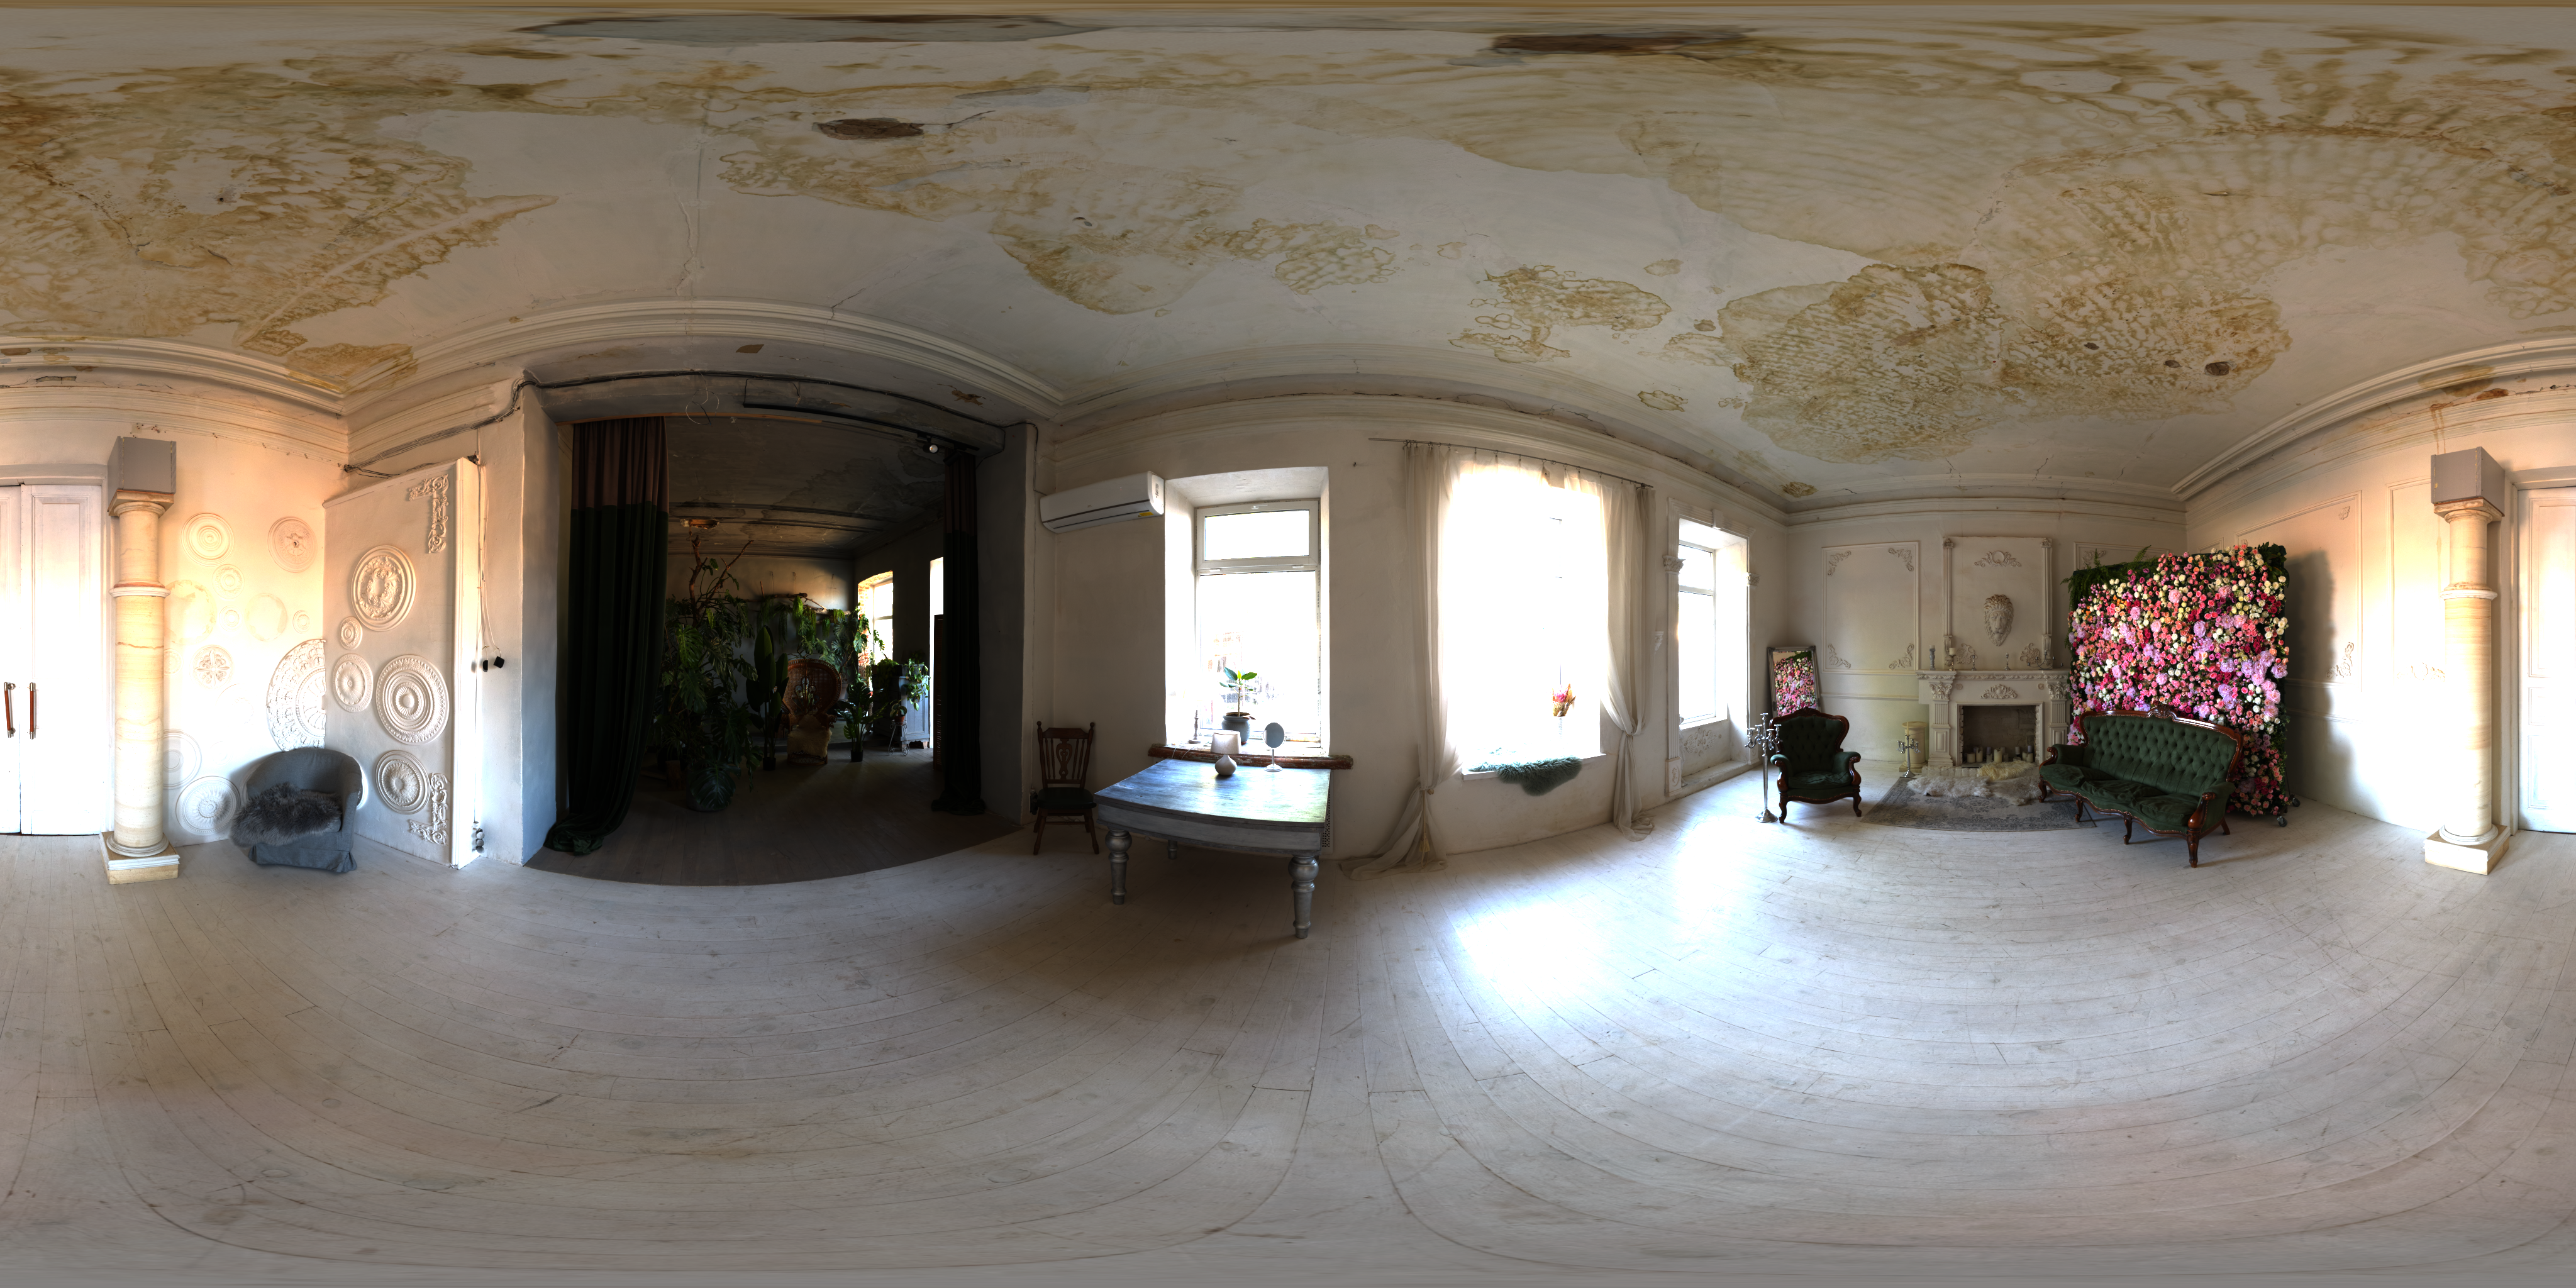
\includegraphics[width=0.45\textwidth]{imgs/photo_studio_london_hall_4k.png}
  \includegraphics[width=0.45\textwidth]{imgs/photo_studio_london_hall_4k-min.png}
  \caption{HDRI \cite{polyhaven2022}}
  \label{fig:hdri}
\end{figure}
\section{Scene}
%% analyzing the real object
The object was placed on a desk in the reference image.

%% describing the implementation
The desk was reconstructed using a simple square patch and textured with a wooden texture taken from Pixar One Twenty Eight \cite{pixar2018} using PxrTexture.
The camera is rotated slightly downwards to show the top of the cap.
\section{Camera Artefacts}
%% analyzing the real object


%% describing the implementation
\input{9.conclusion}

% DO NOT INCLUDE ACKNOWLEDGMENTS IN AN ANONYMOUS SUBMISSION TO SIGGRAPH 2019
% \begin{acks}

% The authors would like to thank Dr. Maura Turolla of Telecom
% Italia for providing specifications about the application scenario.

% The work is supported by the \grantsponsor{GS501100001809}{National
%  Natural Science Foundation of
%  China}{http://dx.doi.org/10.13039/501100001809} under Grant
% No.:~\grantnum{GS501100001809}{61273304\_a}
% and~\grantnum[http://www.nnsf.cn/youngscientists]{GS501100001809}{Young
%  Scientists' Support Program}.


% \end{acks}

% Bibliography
\bibliographystyle{ACM-Reference-Format}
% \bibliography{sample-bibliography}
\bibliography{references}

% Appendix
% \appendix
% \section{Switching Times}

% In this appendix, we measure the channel switching time of Micaz
% \cite{CROSSBOW} sensor devices.  In our experiments, one mote
% alternatingly switches between Channels~11 and~12. Every time after
% the node switches to a channel, it sends out a packet immediately and
% then changes to a new channel as soon as the transmission is finished.
% We measure the number of packets the test mote can send in 10 seconds,
% denoted as $N_{1}$. In contrast, we also measure the same value of the
% test mote without switching channels, denoted as $N_{2}$. We calculate
% the channel-switching time $s$ as
% \begin{displaymath}%
% s=\frac{10}{N_{1}}-\frac{10}{N_{2}}.
% \end{displaymath}%
% By repeating the experiments 100 times, we get the average
% channel-switching time of Micaz motes: 24.3\,$\mu$s.


\end{document}
